\begin{figure}[ht!]
    \centering
    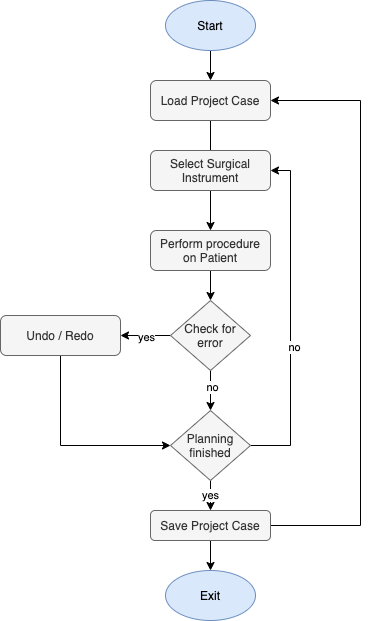
\includegraphics[width=225px]{images/implementation/interaction_flow.png}
    \caption{\label{fig::InteractionFlow} Simplified Flow of Interaction during the Planning Stage}
\end{figure}

The basic flow of interaction for planning a procedure via the software is depicted in Figure \ref{fig::InteractionFlow}.
First, a user has to enable the graphical user interface via the click of a button on the controller.
The user interface will be stuck to the left hand of the user, another click of the button will freeze the GUI in place.
The user interacts with the graphical interface by perfoming virtual button presses with his virtual hands.
Via the interface, the user first chooses a project case he wants to work on.
This will load the patient into the virtual operating room, ready for planning the procedure via the available tools.
From here on, the user can freely choose which procedure to perform and in which order.
Tools can be selected via simply walking or teleporting to them and making a grab motion with the Valve Index controller.
When holding a surgical instrument, the Trigger button has to be pressed to perform the procedure.
By simply touching the Trigger button, the user gets a visual indication that a procedure is about to be performed.
When performing a procedure step, the user gets auditory feedback that the step has been registered.
At any point of performing the procedure, the user can choose to undo and redo the current step via the voice interface.
Only the last performed step will be visible while planning the procedure for visibility reasons.
\newline
Not depicted in the flow chart is the selection of the operating theatre, which is the first scene the user will see when starting the application.
\newline
The training stage, which can be performed after a procedure has been planned, is almost identical to the planning stage.
Here, the user has to follow instructions visible inside of the operating room and perform the planned procedure step by step as he is being told.
Instructions correlate to the planned procedures, but can also be written manually from outside of the application. 
A visual representation of where the user has to perform the step is visible at all times.
The voice feedback will indicate whether the procedure has been performed correctly.
Reasons for errors could be the usage of the wrong surgical instrument or incorrect placement.
\newline
Lastly, when a procedure is planned and the project case has been finished, the user has to save the project via the graphical user interface.
This will create a copy of the current patient model including all procedure steps and save it to the users hard drive.
This way, original data will not be lost and a project can always be redone from scratch.
